\documentclass[a4paper,10pt]{report}
\usepackage[utf8]{inputenc}
\usepackage{hyperref}
\usepackage{graphicx}

\setlength{\parindent}{0mm}
\setlength{\parskip}{2mm}
\setlength{\textwidth}{450pt} %Veränderung des Textblocks in Anpassung an den R Zeilenüberhang bei Aufrufswiederholungen
\setlength{\hoffset}{-50pt} % "
\setlength{\topmargin}{-30pt}
\setlength{\textheight}{670pt}

\setcounter{secnumdepth}{3}
\setcounter{tocdepth}{3}

% Title Page
\title{BRAKER2 User Guide}
\author{Katharina J.~Hoff}


\begin{document}
\maketitle

\tableofcontents

\chapter{Introduction}

\section{What is BRAKER2?}

The rapidly growing number of sequenced genomes requires fully automated methods for accurate gene structure annotation. With this goal in mind, we have developed BRAKER1 \cite{braker1}, a combination of GeneMark-ET \cite{GeneMark-ET} and AUGUSTUS \cite{AUGUSTUS,stanke2006gene}, that uses genomic and RNA-Seq data to automatically generate full gene structure annotations in novel genomes.

However, the quality of RNA-Seq data that is available for annotating a novel genome is variable, and in some cases, RNA-Seq data is not available, at all.

BRAKER2 is an extension of BRAKER1 which allows for \textbf{fully automated training} of the gene prediction tools GeneMark-EX \cite{AlexandreLomsadze11282005,ter2008gene,GeneMark-ET}\footnote{EX = ES/ET/EP/ETP, all available for download under the name \textit{GeneMark-ES/ET}} and AUGUSTUS from RNA-Seq and/or protein homology information, and that integrates the extrinsic evidence from RNA-Seq and protein homology information into the \textbf{prediction}.

In contrast to other available methods that rely on protein homology information, BRAKER2 reaches high gene prediction accuracy even in the absence of the annotation of very closely related species and in the absence of RNA-Seq data. 

BRAKER2 can also combine RNA-Seq and protein homology information.

\section{Keys to successful gene prediction}

\begin{itemize}
 \item Use a high quality genome assembly. If you have a huge number of very short scaffolds in your genome assembly, those short scaffolds will likely increase runtime dramatically but will not increase prediction accuracy. 
 \item Use simple scaffold names in the genome file (e.g.~\texttt{>contig1} will work better than \texttt{>contig1|my custom species name|some putative function|/more/information/ | and lots of special characters \%\^\&!*()\{\}}). Make the scaffold names in all your fasta files simple before running any alignment program.
 \item In order to predict genes accurately in a novel genome, the genome should be masked for repeats. This will avoid the prediction of false positive gene structures in repetitive and low complexitiy regions. Repeat masking is also essential for mapping RNA-Seq data to a genome. In case of GeneMark-EX and AUGUSTUS, softmasking (i.e.~putting repeat regions into lower case letters and all other regions into upper case letters) leads to better results than hardmasking (i.e.~replacing letters in repetitive regions by the letter \texttt{N} for unknown nucleotide). If the genome is masked, use the \texttt{--softmasking} flag of \texttt{braker.pl}.
 
 \item Many genomes have gene structures that will be predicted accurately with standard parameters of GeneMark-EX and AUGUSTUS within BRAKER2. However, some genomes have clade-specific features, i.e.~special branch point model in fungi, or non-standard splice-site patterns. Please read the options section \ref{options} in order to determine whether any of the custom options may improve gene prediction accuracy in the genome of your target species.
 
 \item Always check gene prediction results before further usage! You can e.g.~use a genome browser for visual inspection of gene models in context with extrinsic evidence data.
\end{itemize}

\section{Overview of modes for running BRAKER2}

BRAKER2 mainly features semi-unsupervised, extrinsic evidence data (RNA-Seq and/or protein spliced alignment information) supported training of GeneMark-EX\footnote{EX=ES/ET/EP} and subsequent training of AUGUSTUS with integration of extrinsic evidence in the final gene prediction step. However, there are now a number of additional pipelines included in BRAKER2. In the following, we give an overview of possible input files and pipelines:

\begin{itemize}
 \item genome and RNA-Seq file from the same species (see figure \ref{braker-main}A); this approach is suitable for RNA-Seq libraries with a good coverage of the transcriptome, \textbf{important:} this approach requires that each intron is covered by many alignments, i.e.~it does not work with assembled transcriptome mappings,
 \item genome file and database of proteins that may be of longer evolutionary distance to the target species (see figure \ref{braker-main}B); this approach is suitable if no RNA-Seq data is available, and if no protein data from a very closely related species is available, \textbf{important:} this approach requires a database of protein families, i.e. many representatives of each protein family must be present in the database, please contact Alexandre Lomsadze for information about the required external GaTech protein mapping pipeline,
 \item genome and RNA-Seq file from the same species, and proteins that may be of longer evolutionary distance to the target species (see figure \ref{braker-main}C); \textbf{important:} this approach requires a database of protein families, i.e. many representatives of each protein family must be present in the database,
 \item genome file and file with proteins of short evolutionary distance (see figure \ref{braker2-sidetrack}B); this approach is suitable if RNA-Seq data is not available and if the reference species is very closely related,
 \item genome and RNA-Seq file and proteins of short evolutionary distance (see figures \ref{braker2-sidetrack}A and \ref{braker2-sidetrack}C). In both cases, GeneMark-ET is trained supported by RNA-Seq data, and the resulting gene predictions are used for training AUGUSTUS. In approach A), protein alignment information is used in the gene prediction step with AUGUSTUS, only. In approach C), protein spliced alignment data is used to complement the training set for AUGUSTUS. The latter approach is in particular suitable if RNA-Seq data does not produce a sufficiently high number of training gene structures for AUGUSTUS, and if a very closely related and already annotated species is available.
 \item genome file, only. In this mode, GeneMark-ES is trained on the genome sequence, alone. Long genes predicted by GeneMark-ES are selected for training AUGUSTUS. Final predictions by AUGUSTUS are \textit{ab initio}. This approach will likely yield lower prediction accuracy than all other here described pipelines.
\end{itemize}

\begin{figure}[h!]
	\begin{center}
		\begin{tabular}{c c c c c c c c}
			A) & 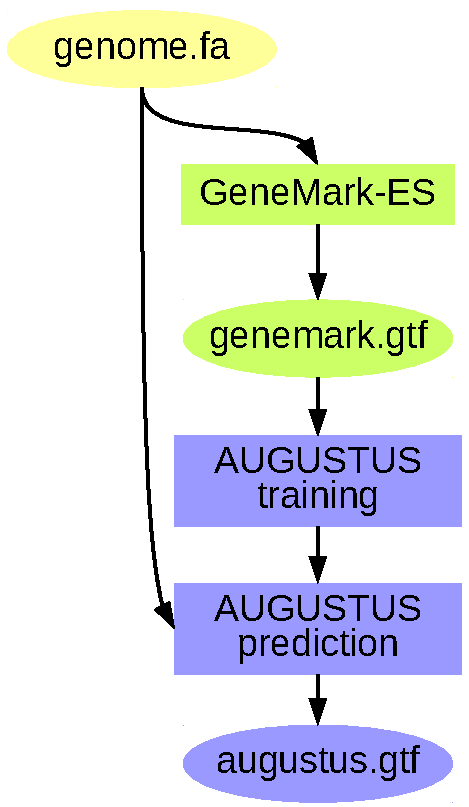
\includegraphics[scale=0.255]{./figs/braker-es.pdf} & B) & 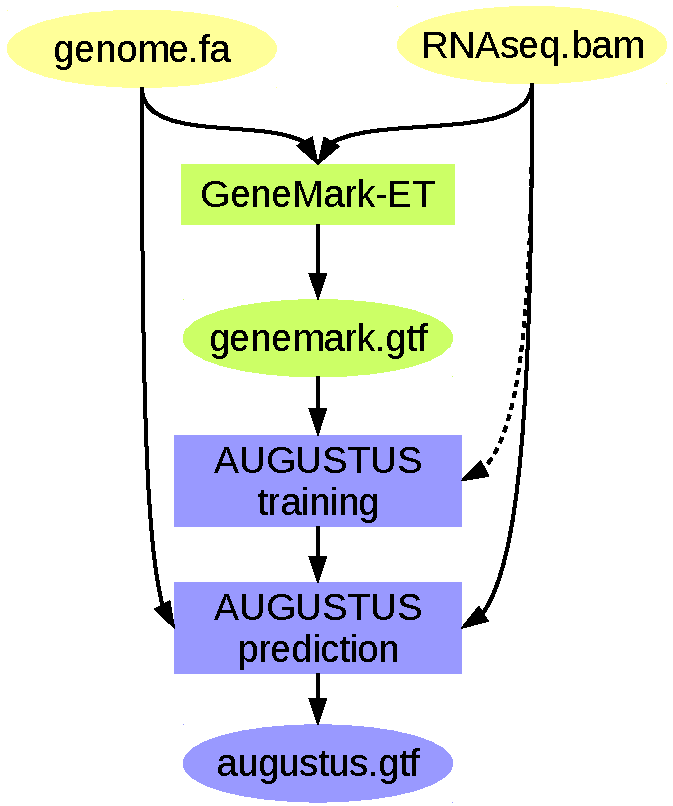
\includegraphics[scale=0.255]{./figs/braker1.pdf} & C) &  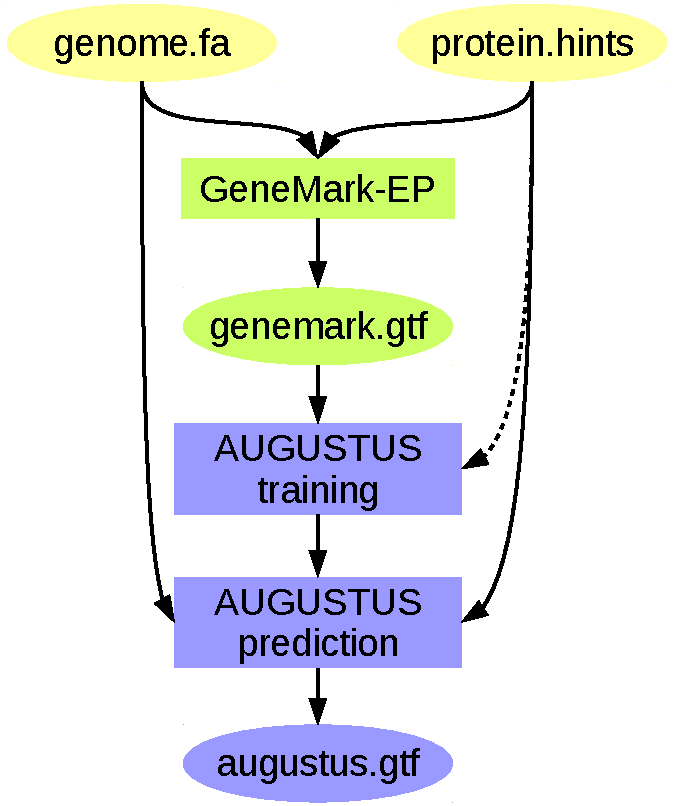
\includegraphics[scale=0.255]{./figs/braker2_ep.pdf} & D) 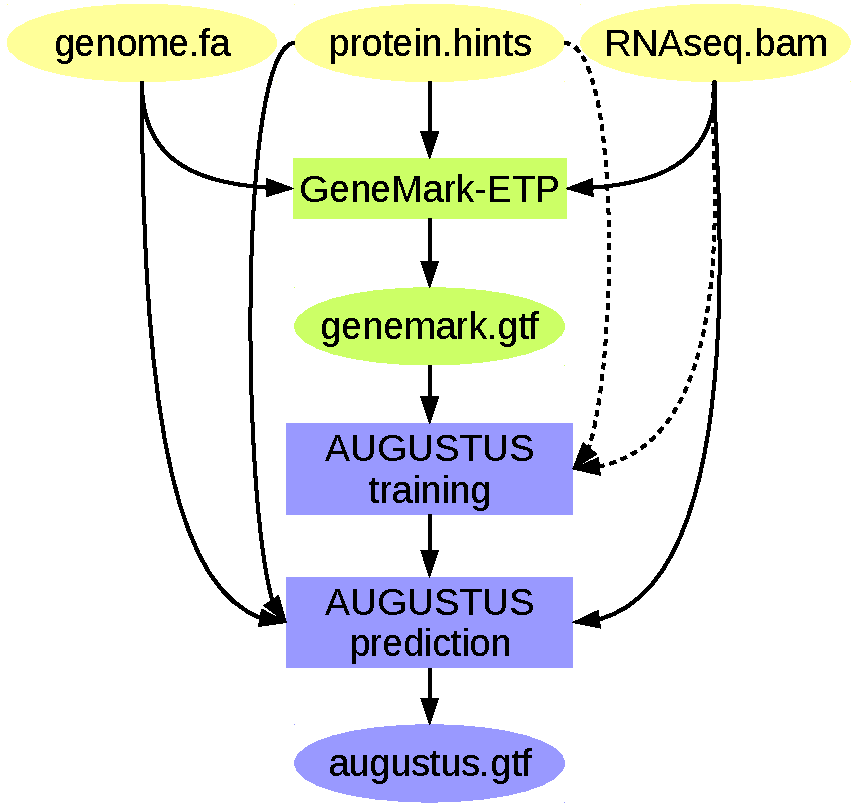
\includegraphics[scale=0.255]{./figs/braker2_ep_rnaseq.pdf}\\
			% braker1.pdf: 323x387 pixel, 72dpi, 11.39x13.65 cm, bb=0 0 323 387
		\end{tabular}
		\caption{BRAKER pipeline: A) training GeneMark-ES on genome data, only; \textit{ab initio} gene prediction with AUGUSTUS, B) training GeneMark-ET supported by RNA-Seq spliced alignment information, prediction with AUGUSTUS with that same spliced alignment information, C) training GeneMark-EP on protein spliced alignment information, prediction with AUGUSTUS with that same spliced alignment information. Proteins used for C) can be of longer evolutionary distance, D) training GeneMark-ETP supported by RNA-Seq alignment information and protein spliced alignment information (proteins can be of longer evolutionary distance), prediction with AUGUSTUS using the same alignment information. Introns supported by both RNA-Seq and protein alignment information are treated as ``true positive introns'', their prediction in gene structures by GeneMark-ETP and AUGUSTUS is enforced.\label{braker-main}}
	\end{center}
\end{figure}

\begin{figure}
\begin{center}
\begin{tabular}{c c c c c c}
 A) & 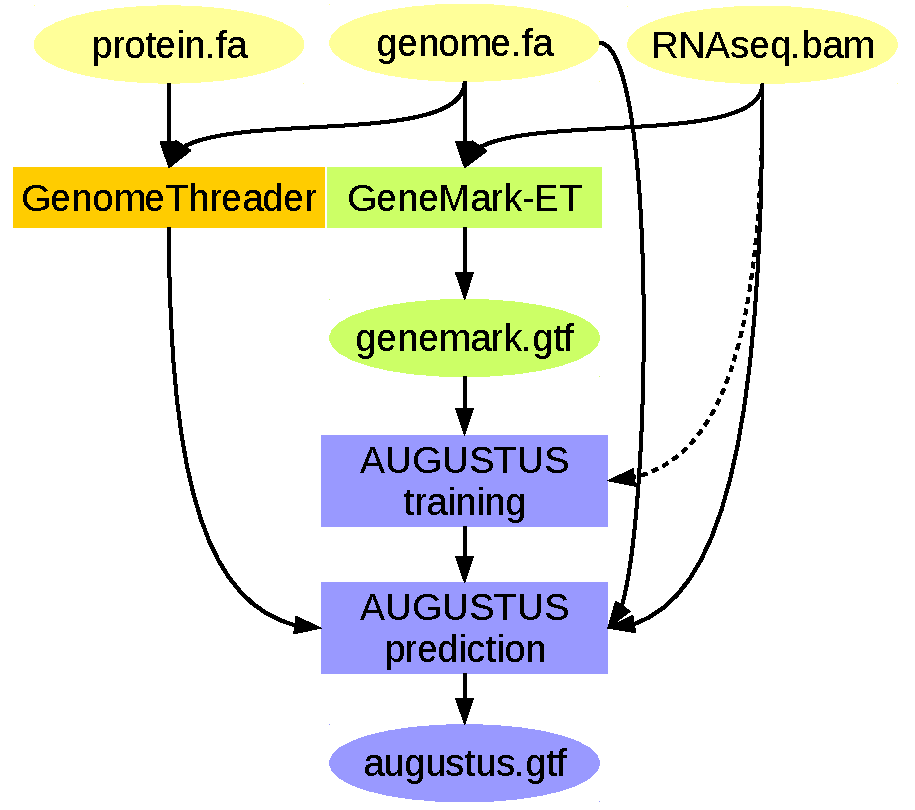
\includegraphics[scale=0.27]{./figs/braker2.pdf} & B) &  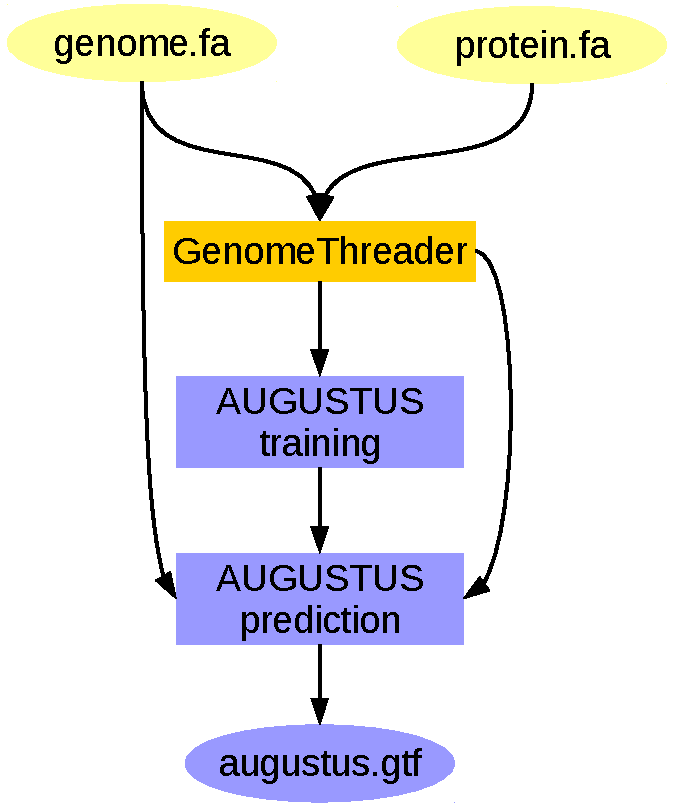
\includegraphics[scale=0.27]{./figs/braker2_gth.pdf} & C) & 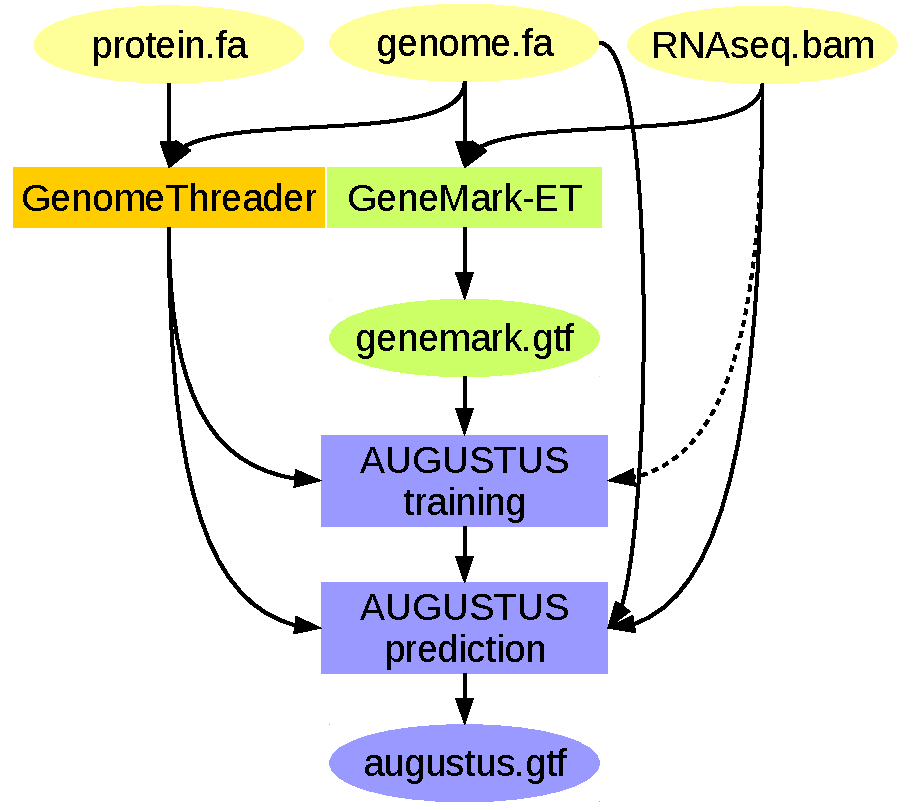
\includegraphics[scale=0.27]{./figs/braker2_train_from_both.pdf}\\
 % braker1.pdf: 323x387 pixel, 72dpi, 11.39x13.65 cm, bb=0 0 323 387
 \end{tabular}
 \caption{Additional pipelines that can be executed by \texttt{braker.pl}: A) training GeneMark-ET supported by RNA-Seq spliced alignment information, prediction with AUGUSTUS with spliced alignment information from RNA-Seq data and with gene features determined by alignments from proteins of a very closely related species against the target genome, B) training AUGUSTUS on the basis of spliced alignment information from proteins of a very closely related species against the target genome, C) training GeneMark-ET on the basis of RNA-Seq spliced alignment information, training AUGUSTUS on a set of training gene structures compiled from RNA-Seq supported gene structures predicted by GeneMark-ET and spliced alignment of proteins of a very closely related species.\label{braker2-sidetrack}}
 \end{center}
 \end{figure} 
 

\chapter{Installation}

\section{Supported software versions}

At the time of release, this BRAKER2 version was tested with:

\begin{itemize}
\item AUGUSTUS 3.3.1\footnote{Please use the latest version of AUGUSTUS distributed by the original developers, it is available from github at \url{https://github.com/Gaius-Augustus/Augustus}. Problems have been reported from users that tried to run BRAKER with AUGUSTUS releases maintained by third parties, i.e. Bioconda.}
   \item  GeneMark-ET 4.33
   \item  BAMTOOLS 2.5.1 \cite{barnett2011bamtools}
   \item  SAMTOOLS 1.7-4-g93586ed \cite{li2009sequence}
   \item  GenomeThreader 1.7.0 \cite{gremme2013}
   \item  (Spaln 2.3.1 \cite{gotoh2008direct,gotoh2008space,iwata2012benchmarking})\footnote{Not tested in this release, we recommend using GenomeThreader, instead}
   \item  (Exonerate 2.2.0 \cite{slater2005automated})\footnote{Not tested in this release, we recommend using GenomeThreader, instead}
   \item  NCBI BLAST+ 2.2.31+ \cite{Altschul:1990,camacho2009blast+}
\end{itemize}

\section{BRAKER2}

\subsection{Perl pipeline dependencies}

Running BRAKER2 requires a Linux-system with \texttt{bash} and Perl. Furthermore, BRAKER2 requires the following CPAN-Perl modules to be installed:

\begin{itemize}
 \item 		  \texttt{File::Spec::Functions}
				\item \texttt{Hash::Merge}
				\item \texttt{List::Util}
				\item \texttt{Logger::Simple}
				\item \texttt{Module::Load::Conditional}
				\item \texttt{Parallel::ForkManager}
				\item \texttt{POSIX}
				\item \texttt{Scalar::Util::Numeric}
				\item \texttt{YAML}
\end{itemize}

   	On Ubuntu, for example, install the modules with CPANminus\footnote{install with \texttt{sudo apt-get install cpanminus}}: \texttt{sudo cpanm [Module::Name]}, e.g. \texttt{sudo cpanm Hash::Merge}.

   BRAKER2 also uses a Perl module \texttt{helpMod.pm} that is not available on CPAN. This module is 
   part of the BRAKER2 release and does not require separate installation.  

\subsection{BRAKER2 components} \label{Executability}

BRAKER2 is a collection of Perl scripts and a Perl module. The main script that will be called in order to run BRAKER2 is \texttt{braker.pl}. Additional Perl components are:

\begin{itemize}
\item \texttt{align2hints.pl}
\item \texttt{filterGenemark.pl}
\item \texttt{filterIntronsFindStrand.pl}
\item \texttt{startAlign.pl}
\item \texttt{helpMod.pm}
\item \texttt{findGenesInIntrons.pl}
\item \texttt{downsample\_traingenes.pl}
\end{itemize}

All Perl scripts (files ending with \texttt{*.pl}) that are part of BRAKER2 must be executable in order to run BRAKER2. This should already be the case if you download BRAKER2 from our website. Executability may be overwritten if you e.g.~transfer BRAKER2 on a USB-stick to anothre computer. In order to check whether required files are executable, run the following command in the directory that contains BRAKER2 Perl scripts:

\begin{verbatim}
ls -l *.pl
\end{verbatim}

The output should be similar to this:

\begin{verbatim}
-rwxr-xr-x 1 katharina katharina  18191 Mai  7 10:25 align2hints.pl
-rwxr-xr-x 1 katharina katharina 408782 Aug 17 18:24 braker.pl
-rwxr-xr-x 1 katharina katharina   5024 Mai  7 10:25 downsample_traingenes.pl
-rwxr-xr-x 1 katharina katharina  30453 Mai  7 10:25 filterGenemark.pl
-rwxr-xr-x 1 katharina katharina   5754 Mai  7 10:25 filterIntronsFindStrand.pl
-rwxr-xr-x 1 katharina katharina   7765 Mai  7 10:25 findGenesInIntrons.pl
-rwxr-xr-x 1 katharina katharina  41674 Mai  7 10:25 startAlign.pl
\end{verbatim}

It is important that the \texttt{x} in \texttt{-rwxr-xr-x} is present for each script. If that is not the case, run

\begin{verbatim}
chmod a+x *.pl
\end{verbatim}

in order to change file attributes.

You may find it helpful to add the directory in which BRAKER2 perl scripts reside to 
    your \texttt{\$PATH} environment variable. For a single bash session, enter:

    \begin{verbatim}
    PATH=/your_path_to_braker/:$PATH
    export PATH
    \end{verbatim}
    
To make this \texttt{\$PATH} modification available to all bash sessions, add the above lines to a startup script (e.g.\texttt{$\sim$/.bashrc}).

\section{Bioinformatics software dependencies}

BRAKER2 calls upon various bioinformatics software tools that are not part of BRAKER2. Some tools are obligatory, i.e.~BRAKER2 will not run at all if these tools are not present on your system. Other tools are optional. Please install all tools that are required for running BRAKER2 in the mode of your choice.

\subsection{Mandatory tools}

\subsubsection{GeneMark-EX}

Download GeneMark-EX\footnote{EX=ES/ET/EP/ETP, available as \textit{GeneMark-ES/ET}} from \url{http://exon.gatech.edu/GeneMark/license_download.cgi}.
 Unpack and install GeneMark-EX as described in GeneMark-EX's \texttt{README} file.

If already contained in your \texttt{\$PATH} variable, BRAKER2 will guess the location of \texttt{gmes\_petap.pl}, automatically. Otherwise, BRAKER2 can find GeneMark-EX executables either by locating them in an environment variable \texttt{GENEMARK\_PATH}, or by taking a command line argument\\ (\texttt{--GENEMARK\_PATH=/your\_path\_to\_GeneMark-EX/gmes\_petap/}). 

In order to set the environment variable for your current Bash session, type: 

    \begin{verbatim}
    export GENEMARK_PATH=/your_path_to_GeneMark-ET/gmes_petap/
\end{verbatim}

Add the above lines to a startup script (e.g.~\texttt{$\sim$/.bashrc}) in order to make it available to all bash sessions.\footnote{GeneMark-EX is not a mandatory tool if AUGUSTUS is to be trained from GenomeThreader aligments with the option \texttt{--trainFromGth}.}


\subsubsection{AUGUSTUS}

Download AUGUSTUS from \url{https://github.com/Gaius-Augustus/Augustus}.
 Unpack AUGUSTUS and install AUGUSTUS  according to AUGUSTUS \texttt{README.TXT}. 
 
You should compile AUGUSTUS on your own system in order to avoid problems with versions of libraries used by AUGUSTUS. Compilation instructions are provided in the AUGUSTUS \texttt{README.TXT} file
   (\texttt{Augustus/README.txt}).

AUGUSTUS consists of \texttt{augustus}, the gene prediction tool, additional C++ tools located in\\ \texttt{augustus/auxprogs} and Perl scripts located in \texttt{augustus/scripts}. Perl scripts must be executable (see instructions in section \ref{Executability} on page \pageref{Executability}). 
   
   The C++ tool \texttt{bam2hints} is an essential component of BRAKER2. Sources are located in \\\texttt{Augustus/auxprogs/bam2hints}. Make sure that you compile \texttt{bam2hints} on your system (it should be automatically compiled when AUGUSTUS is compiled, but in case of problems with \texttt{bam2hints}, please read troubleshooting instructions in 
   \texttt{Augustus/auxprogs/bam2hints/README}).
   
   If you would like to train UTR parameters and integrate RNA-Seq coverage information into gene prediction with BRAKER2 (which is possible only if an RNA-Seq bam-file is provided as extrinsic evidence), \texttt{utrrnaseq} and \texttt{bam2wig} in the \texttt{auxprogs} directory are also required. If compilation with the default \texttt{Makefile} fails, please read troubleshooting instructions in \texttt{Augustus/auxprogs/bam2wig/README.txt} and \texttt{Augustus/auxprogs/utrrnaseq/README}, respectively.
   
   Since BRAKER2 is a pipeline that trains AUGUSTUS, i.e.~writes species specific parameter files, BRAKER2 needs writing access to the configuration directory of AUGUSTUS that contains such files  (\texttt{Augustus/config/}). If you install AUGUSTUS
   globally on your system, the \texttt{config} folder will typically not be writable by all users. Either make the directory where \texttt{config} resides recursively writable to users of AUGUSTUS, or copy the \texttt{config/} folder (recursively) to a location where users have writing permission. 
   
   AUGUSTUS will locate the \texttt{config} folder by looking for an environment variable \texttt{\$AUGUSTUS\_CONFIG\_PATH}. If the \texttt{\$AUGUSTUS\_CONFIG\_PATH} environment variable is not set, then BRAKER2 will look in 
    the path \texttt{../config} relative to the directory in which it finds an AUGUSTUS executable. Alternatively, you can supply the variable as a command line argument to BRAKER2\\ (\texttt{--AUGUSTUS\_CONFIG\_PATH=/your\_path\_to\_AUGUSTUS/augustus/config/}). We recommend that you export the variable e.g.~for your current bash session:

    \begin{verbatim}
    export AUGUSTUS_CONFIG_PATH=/your_path_to_AUGUSTUS/augustus/config/
    \end{verbatim}

In order to make the variable available to all Bash sessions, add the above line to a startup script, e.g.~\texttt{$\sim$/.bashrc}.

\paragraph{Important: } BRAKER2 expects the entire \texttt{config} directory of AUGUSTUS at \texttt{\$AUGUSTUS\_CONFIG\_PATH}, i.e.~the subfolders \texttt{species} with its contents (at least \texttt{generic}) and \texttt{extrinsic}! Providing an writable but empty folder at \texttt{\$AUGUSTUS\_CONFIG\_PATH} will not work for BRAKER. If you need to separate augustus binary and \texttt{\$AUGUSTUS\_CONFIG\_PATH}, we recommend that you recursively copy the un-writable config contents to a writable location.

\noindent \underline{Example:}\\

You have a system-wide installation of AUGUSTUS at \texttt{/usr/bin/augustus}, an unwritable copy of \texttt{config} sits at \texttt{/usr/bin/augustus\_config/}. The folder \texttt{/home/yours/} is writable to you. Copy with the following command (and additionally set the then required variables):\\

\begin{verbatim}
cp -r \texttt{/usr/bin/augustus_config/ /home/yours/
export AUGUSTUS_CONFIG_PATH=/home/yours/augustus_config
export AUGUSTUS_BIN_PATH=/usr/bin
export AUGUSTUS_SCRIPTS_PATH=/usr/bin/augustus_scripts
\end{verbatim}


   
   \paragraph{Modification of \texttt{\$PATH}.} Adding adding directories of AUGUSTUS binaries and scripts to your \texttt{\$PATH} variable enables your system to locate these tools, automatically. It is not a requirement for running BRAKER2 to do this, because BRAKER2 will try to guess them from the location of another environment variable (\texttt{\$AUGUSTUS\_CONFIG\_PATH}), or both directories can be supplied as command line arguments to \texttt{braker.pl}, but we recommend to add them to your \texttt{\$PATH} variable. For your current bash session, type:

    \begin{verbatim}
    PATH=:/your_path_to_augustus/bin/:/your_path_to_augustus/scripts/:$PATH
    export PATH
    \end{verbatim}

    For all your BASH sessions, add the above lines to a startup script (e.g.\texttt{$\sim$/.bashrc}).

   

\subsubsection{Bamtools}

Download BAMTOOLS (e.g.~\texttt{git clone \url{https://github.com/pezmaster31/bamtools.git}}). Install BAMTOOLS by typing the following in your shell:\\

 \begin{verbatim}
   cd your-bamtools-directory
   mkdir build
   cd build
   cmake ..
   make
 \end{verbatim}

 If already in your \texttt{\$PATH} variable, BRAKER2 will find bamtools, automatically. Otherwise, BRAKER2 can locate the bamtools binary either by using an environment variable \texttt{\$BAMTOOLS\_PATH}, or by taking a command line argument (\texttt{--BAMTOOLS\_PATH=/your\_path\_to\_bamtools/bin/}\footnote{The binary may e.g.~reside in bamtools/build/src/toolkit}). In order to set the environment variable e.g.~for your current bash session, type:

    \begin{verbatim}
        export BAMTOOLS_PATH=/your_path_to_bamtools/bin/ 
    \end{verbatim} 

    Add the above line to a startup script (e.g.~\texttt{$\sim$/.bashrc}) in order to set the environment variable for all bash sessions.

    
\subsubsection{NCBI BLAST+}

On Ubuntu, install with \texttt{sudo apt-get install ncbi-blast+}.

If already in your \texttt{\$PATH} variable, BRAKER2 will find blastp, automatically. Otherwise, BRAKER2 can locate the blastp binary either by using an environment variable \texttt{\$BLAST\_PATH}, or by taking a command line argument (\texttt{--BLAST\_PATH=/your\_path\_to\_blast/}). In order to set the environment variable e.g.~for your current bash session, type:

    \begin{verbatim}
        export BLAST_PATH=/your_path_to_blast/ 
    \end{verbatim} 

    Add the above line to a startup script (e.g.~\texttt{$\sim$/.bashrc}) in order to set the environment variable for all bash sessions.




\subsection{Optional tools}

\subsubsection{Samtools}

Samtools is not required for running BRAKER2 if all your files are formatted, correctly (i.e.~all sequences should have short and unique fasta names). If you are not sure
      whether all your files are fomatted correctly, it might be helpful to have Samtools
      installed because BRAKER2 can automatically fix certain format issues by using Samtools. 

      As a prerequisite for Samtools, download and install \texttt{htslib} (e.g.~ 
      \texttt{git clone \url{https://github.com/samtools/htslib.git}}, follow the \texttt{htslib} documentation for 
      installation).

      Download and install Samtools (e.g. \texttt{git clone \url{git://github.com/samtools/samtools.git}}), 
      subsequently follow Samtools documentation for installation).    

      If already in your \texttt{\$PATH} variable, BRAKER2 will find samtools, automatically. Otherwise, BRAKER2 can find Samtools either by taking a command line argument\\ (\texttt{--SAMTOOLS\_PATH=/your\_path\_to\_samtools/}), or by using an environment variable \texttt{\$SAMTOOLS\_PATH}. For exporting the variable, e.g.~for your current bash session, type:

    \begin{verbatim}
      export SAMTOOLS_PATH=/your_path_to_samtools/
    \end{verbatim}
    
        Add the above line to a startup script (e.g.~\texttt{$\sim$/.bashrc}) in order to set the environment variable for all bash sessions.
        
\subsubsection{Python3 \& Biopython}

If Python3 and Biopython are installed, BRAKER2 can generate FASTA-files with coding sequences and protein sequences predicted by AUGUSTUS. This is an optional step, it can be disabled with the command-line flag \texttt{-{}-skipGetAnnoFromFasta}; Python3 and Biopython are not required if this flag is set.

On Ubuntu, Python3 is installed by default. Install the Python3 package manager with:

\begin{verbatim}
sudo apt-get install python3-pip
\end{verbatim}

Subsequently, install Biopython with:

\begin{verbatim}
sudo pip3 install biopython
\end{verbatim}

On Ubuntu, python3 will be in your \$PATH variable, by default, and BRAKER2 will automatically locate it. However, you have the option to specify the \texttt{python3} binary location in two other ways:

\begin{enumerate}
\item Export an environment variable \texttt{\$PYTHON3\_PATH}, e.g.~in your \texttt{$\sim$/.bashrc} file:
\begin{verbatim}
export PYTHON3_PATH=/path/to/python3/
\end{verbatim}
\item Specify the command line option \texttt{-{}-PYTHON3\_PATH=/path/to/python3/} to \texttt{braker.pl}.
\end{enumerate}


\subsubsection{GenomeThreader}

This tool is required, only, if you would like to run protein to genome alignments with BRAKER2 using GenomeThreader. This is a suitable approach if an annotated species of short evolutionary distance to your target genome is available. Download GenomeThreader from \url{http://genomethreader.org/}. Unpack and install according to \texttt{gth/README}.

BRAKER2 will try to locate the GenomeThreader executable by using an environment variable\\\texttt{\$ALIGNMENT\_TOOL\_PATH}. Alternatively, this can be supplied as command line argument \\(\texttt{--ALIGNMENT\_TOOL\_PATH=/your/path/to/gth}).

\subsubsection{Spaln}

This tool is required, only, if you would like to run protein to genome alignments with BRAKER2 using Spaln. This is a suitable approach if an annotated species of short evolutionary distance to your target genome is available. (We recommend the usage of GenomeThreader instad of Spaln.) Download Spaln from \url{http://www.genome.ist.i.kyoto-u.ac.jp/~aln_user}. Unpack and install according to \texttt{spaln/doc/SpalnReadMe22.pdf}.

BRAKER2 will try to locate the Spaln executable by using an environment variable \texttt{\$ALIGNMENT\_TOOL\_PATH}. Alternatively, this can be supplied as command line argument \\(\texttt{--ALIGNMENT\_TOOL\_PATH=/your/path/to/spaln}).

\subsubsection{Exonerate}

This tool is required, only, if you would like to run protein to genome alignments with BRAKER2 using Exonerate. This is a suitable approach if an annotated species of short evolutionary distance to your target genome is available. (We recommend the usage of GenomeThreader instad of Exonerate because Exonerate is comparably slower and has lower specificity than GenomeThreader.) Download Exonerate from \url{https://github.com/nathanweeks/exonerate}. Unpack and install according to \texttt{exonerate/README}. (On Ubuntu, download and install by typing  \texttt{sudo apt-get install exonerate}.)

BRAKER2 will try to locate the Exonerate executable by using an environment variable \\\texttt{\$ALIGNMENT\_TOOL\_PATH}. Alternatively, this can be supplied as command line argument \\(\texttt{--ALIGNMENT\_TOOL\_PATH=/your/path/to/exonerate}).

\chapter{Running BRAKER2}

\section{Different BRAKER2 pipeline modes}

In the following, we describe ``typical'' BRAKER2 calls for different input data types. In general, we recommend that you run BRAKER2 on genomic sequences that have been softmasked for Repeats. If your genome has been softmasked, include the \texttt{--softmasking} flag in your BRAKER2 call!

\subsection{BRAKER2 with RNA-Seq data (only)}\label{braker1}.

This approach is suitable for genomes of species for which RNA-Seq libraries with a good coverage of the transcriptome are available. The pipeline is illustrated in figure \ref{braker-main}A) on page \pageref{braker-main}.

BRAKER2 can either extract RNA-Seq spliced alignment information from \texttt{bam} files, or it can use such extracted information, directly.

In order to run BRAKER2 with RNA-Seq data supplied as \texttt{bam} file(s) (in case of multiple files, separate them by comma), run:

\begin{verbatim}
   braker.pl --species=yourSpecies --genome=genome.fasta --bam=file1.bam,file2.bam
\end{verbatim}

In order to run BRAKER2 with RNA-Seq spliced alignment information that has already been extracted, run:

\begin{verbatim}
   braker.pl --species=yourSpecies --genome=genome.fasta \
      --hints=hints1.gff,hints2.gff
\end{verbatim}

The format of such a hints file must be as follows (tabulator separated file):

\begin{verbatim}
chrName	b2h	intron	6591	8003	1	+	.	pri=4;src=E
chrName	b2h	intron	6136	9084	11	+	.	mult=11;pri=4;src=E
...
\end{verbatim}

The source \texttt{b2h} in the second column and the source tag \texttt{src=E} in the last column are essential for BRAKER2 to determine whether a hint has been generated from RNA-Seq data. 

\subsubsection{Training and prediction of UTRs, integration of coverage information}

If RNA-Seq (and only RNA-Seq) data is provided to BRAKER2 as a bam-file, and if the genome is softmasked for repeats, BRAKER2 can automatically train UTR parameters for AUGUSTUS. After successful training of UTR parameters, BRAKER2 will automatically predict genes including coverage information form RNA-Seq data. Example call:

\begin{verbatim}
   braker.pl --species=yourSpecies --genome=genome.fasta --bam=file.bam --softmasking \
      --UTR=on
\end{verbatim}

\subsubsection{Stranded RNA-Seq alignments}

For running BRAKER2 without UTR paramters, it is not very important whether RNA-Seq data was generated by a \textit{stranded} protocol (because spliced alignments are 'artificially stranded' by checking the splice site pattern). However, for UTR training and prediction, stranded libraries may provide information that is valuable for BRAKER2.

After alignment of the stranded RNA-Seq libraries, separate the resulting bam file entries into two files: one for plus strand mappings, one for minus strand mappings. Call BRAKER2 as follows:

\begin{verbatim}
   braker.pl --species=yourSpecies --genome=genome.fasta --softmasking \
      --bam=plus.bam,minus.bam --stranded=+,- --UTR=on
\end{verbatim}

You may additionally include bam files from unstranded libraries. Those files will not used for generating UTR training examples, but they will be included in the final gene prediction step as unstranded coverage information, example call:

\begin{verbatim}
   braker.pl --species=yourSpecies --genome=genome.fasta --softmasking \
      --bam=plus.bam,minus.bam,unstranded.bam --stranded=+,-,. --UTR=on
\end{verbatim}

\subsection{BRAKER2 with proteins of longer evolutionary distance}

This approach is suitable for genomes of species for which no RNA-Seq libraries are available and for which no closely related and well annotated genome is available. A database of proteins with longer evolutionary distance to the target species may be used in this case. The pipeline is illustrated in figure \ref{gatech} on page \pageref{gatech}.

\begin{figure}
 \centering
 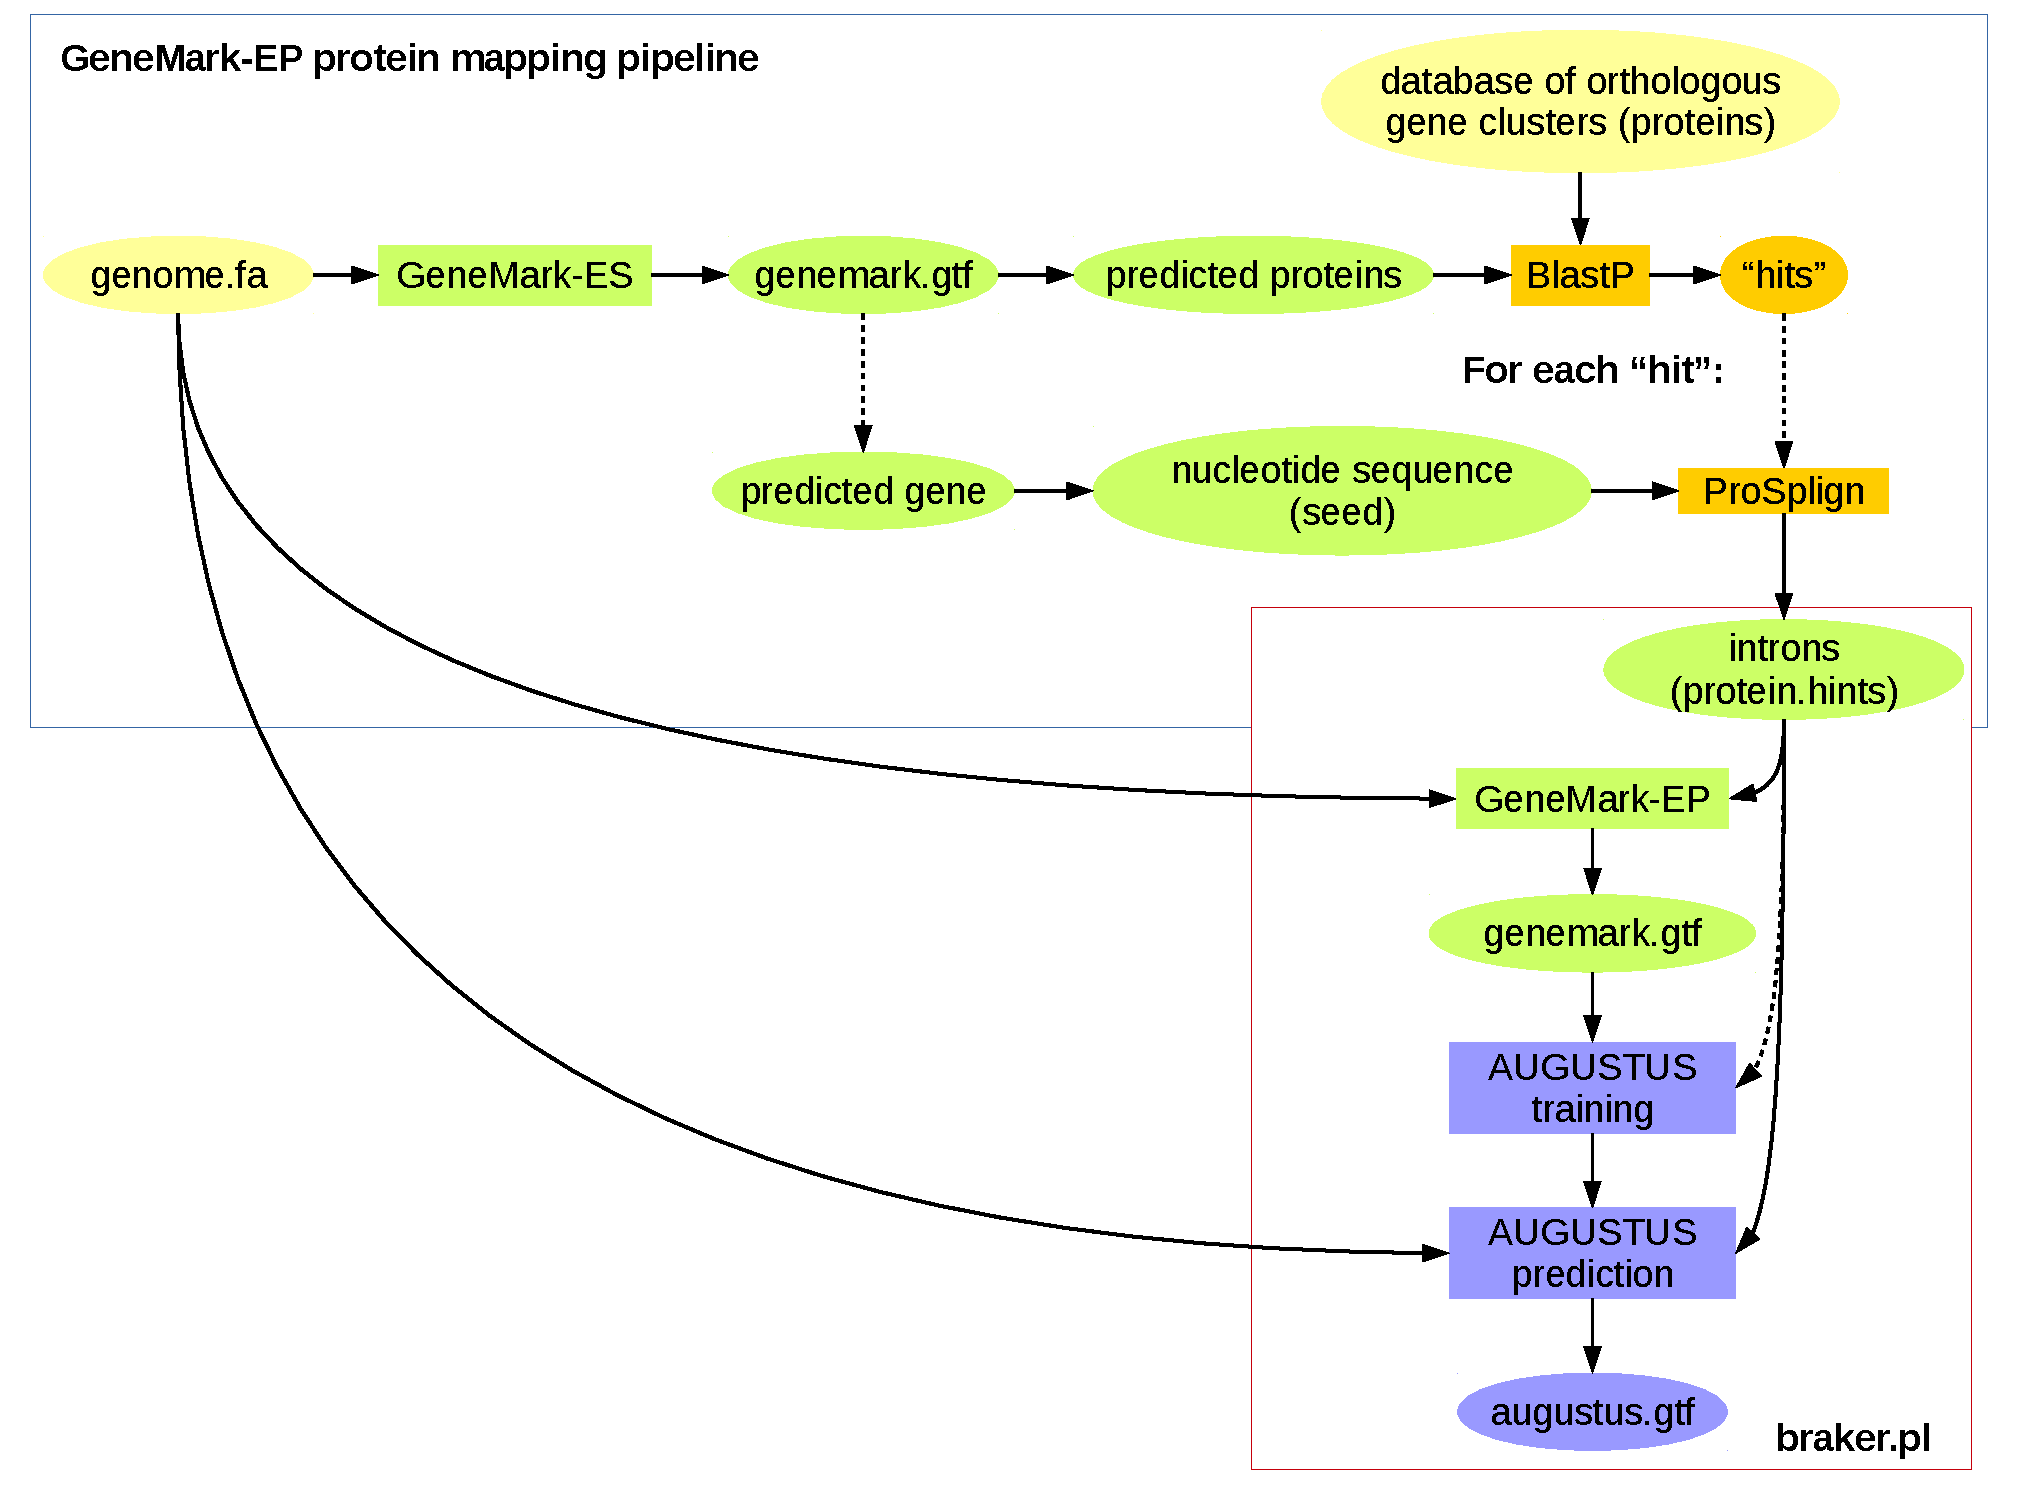
\includegraphics[scale=0.4]{./figs/gatech-prot-pipeline.pdf}
 --hints=hints.gff --epmode
 % gatech-prot-pipeline.pdf: 972x713 pixel, 72dpi, 34.29x25.15 cm, bb=0 0 972 713
 \caption{BRAKER2 and GeneMark-EP protein mapping pipeline.}
 \label{gatech}
\end{figure}

Running BRAKER2 with proteins of longer evolutionary distance requires the preparation of ``protein hints'' before running BRAKER2, itself. Preparing protein hints is in this case not part of BRAKER2 because in contrast to BRAKER2, which can run on a work station with one or multiple cores, the GeneMark-EP specific protein mapping pipeline requires a cluster for execution. Please contact Alexandre Lomsadze for more information about the protein mapping pipeline.

For running BRAKER2 in this mode, type:

\begin{verbatim}
   braker.pl --species=yourSpecies --genome=genome.fasta \
\end{verbatim}

The format of such a hints file must be as follows (tabulator separated file):

\begin{verbatim}
chrName	ProSplign	intron	6591	8003	5	+	.	mult=5;pri=4;src=P
chrName	ProSplign	intron	6136	9084	11	+	.	mult=11;pri=4;src=P
...
\end{verbatim}

The source \texttt{ProSplign} in the second column and the source tag \texttt{src=P} in the last column are essential for BRAKER2 to determine whether a hint has been generated from remote homology protein data. 

\subsection{BRAKER2 with proteins of shorter evolutionary distance}\label{prot-in}

This approach is suitable if RNA-Seq data for the species of the target genome is not available and if a well annotated and very closely related reference species is available. The pipeline is illustrated in figure \ref{braker2-sidetrack}B) on page \pageref{braker2-sidetrack}.

For running BRAKER2 in this mode, type:

\begin{verbatim}
   braker.pl --species=yourSpecies --genome=genome.fasta \
      --prot_seq=proteins.fa --prg=gth --ALIGNMENT_TOOL_PATH=/path/to/gth/binary \
      --trainFromGth
\end{verbatim}

It is possible to generate protein alignments externally, prior running BRAKER2, itself. The compatible command for running GenomeThreader prior running BRAKER2, is:

\begin{verbatim}
   gth -genomic genome.fa  -protein protein.fa -gff3out -skipalignmentout -o gth.aln
\end{verbatim}


In order to use such externally created alignment files, run:

\begin{verbatim}
   braker.pl --species=yourSpecies --genome=genome.fasta \
      --prot_aln=proteins.aln --prg=gth --trainFromGth
\end{verbatim}

It is also possible to run BRAKER2 in this mode using an already prepared hints file. In this case, run:

\begin{verbatim}
   braker.pl --species=yourSpecies --genome=genome.fasta \
      --hints=hints.gff --prg=gth --trainFromGth
\end{verbatim}

Format of the hints file should look like this:

\begin{verbatim}
chrName   gth2h   CDSpart 105984  106633  .     -    .    src=P;grp=FBpp0285205;pri=4
chrName   gth2h   start   106646  106648  .     -    .    src=P;grp=FBpp0285205;pri=4
\end{verbatim}

Supported features are intron, CDSpart, start, stop.

\subsection{BRAKER2 with RNA-Seq and protein data}

BRAKER2 with RNA-Seq and protein data is currently still under development. BRAKER2 currently does not train GeneMark-EX from protein and RNA-Seq data, yet. However, if RNA-Seq data of the target species and protein data of a very closely related reference species are available, BRAKER2 already supports the following to modes.

\subsubsection{Adding protein data of short evolutionary distance to gene prediction step}

This pipeline is illustrated in figure \ref{braker2-sidetrack}A) on page \pageref{braker2-sidetrack}.

In general, add the options

\begin{verbatim}
   --prot_seq=proteins.fa --prg=(gth|exonerate|spaln)
\end{verbatim}

to the BRAKER2 call that is described in section \ref{braker1}. Select one protein alignment tool from GenomeThreader (\texttt{gth}, recommended), Spaln (\texttt{spaln}) or Exonerate (\texttt{exonerate}). Of course, you may also specify the protein information as protein alignment files or hints files as described in section \ref{prot-in} on page \pageref{prot-in}). This may result in a call similar to:

\begin{verbatim}
   braker.pl --species=yourSpecies --genome=genome.fasta --bam=file1.bam,file2.bam \
      --prot_seq=proteins.fa --prg=(gth|exonerate|spaln)
\end{verbatim}

\subsubsection{Extending training gene set with proteins of short evolutionary distance}

If the number of training gene structures identified by RNA-Seq data, only, seems to be too small, you may add training gene structures generated by protein alignments with GenomeThreader to the training gene set. This pipeline is illustrated in \ref{braker2-sidetrack}C) on page \pageref{braker2-sidetrack}.

In general, add the options

\begin{verbatim}
   --prot_seq=proteins.fa --prg=gth --gth2traingenes
\end{verbatim}

to the BRAKER2 call that is described in section \ref{braker1}. This may result in a call similar to:

\begin{verbatim}
   braker.pl --species=yourSpecies --genome=genome.fasta --bam=file1.bam,file2.bam \
      --prot_seq=proteins.fa --prg=gth --gth2traingenes
\end{verbatim}

\section{Description of selected BRAKER2 command line options}\label{options}

Please run \texttt{braker.pl --help} to obtain a full list of options.

\subsection{\texttt{--ab\_initio}}

Compute AUGUSTUS \textit{ab initio} predictions in addition to AUGUSTUS predictions with hints (additional output files: \texttt{augustus.ab\_initio.*}. This may be useful for estimating the quality of training gene parameters when inspecting predictions in a Browser.

\subsection{\texttt{--augustus\_args=``--some\_arg=bla''}}     
One or several command line arguments to be passed to AUGUSTUS, if several arguments are given, separated by whitespace, i.e.~\texttt{``--first\_arg=sth --second\_arg=sth''}. This may be be useful if you know that gene prediction in your particular species benefits from a particular AUGUSTUS argument during the prediction step.  
    
\subsection{\texttt{--cores=INT}}                              Specifies the maximum number of cores that can be used during computation. BRAKER2 has to run some steps on a single core, others can take advantage of multiple cores. The optimal core number of all steps is 8. If you use more than 8 cores, this will not speed up all parallelized steps, in particular, the time consuming \texttt{optimize\_augustus.pl} will not use more than 8 cores. However, if you don't mind some cores being idle, using more than 8 cores will speed up other steps.
\subsection{\texttt{--fungus}}                             GeneMark-EX option: run algorithm with branch point model. Use this option if you genome is a fungus.
    \subsection{\texttt{--softmasking}}                        Softmasking option for soft masked genome files. (Disabled by default.)
   
    \subsection{\texttt{--useexisting}}                        Use the present config and parameter files if they exist for 
                                         'species'. This step will skip training AUGUSTUS and instead use pre-trained parameters.
  
    \subsection{\texttt{--crf}}                                Execute CRF training for AUGUSTUS; resulting parameters are only kept for
                                         final predictions if they show higher accuracy than HMM parameters. This increases runtime!
    \subsection{\texttt{--lambda=int}}
    Change the parameter $\lambda$ of the Poisson distribution that is used for downsampling training genes according to their number of introns (only genes with up to 5 introns are downsampled). The default value is $\lambda=2$. You might want to set it to 0 for organisms that mainly have single-exon genes. (Generally, single-exon genes contribute less value to increasing AUGUSTUS parameters compared to genes with many exons.)
              
\subsection{\texttt{--UTR=on}} Generate UTR training examples for AUGUSTUS from RNA-Seq coverage information, train AUGUSTUS UTR parameters and predict genes with AUGUSTUS and UTRs, including coverage information for RNA-Seq as evidence. This flag only works if --softmasking is also enabled, and if the only extrinsic evidence provided are bam files.

\subsection{\texttt{--stranded=+,-,.,...}} If \texttt{--UTR=on} is enabled, strand-separated bam-files can be provided with \texttt{--bam=plus.bam,minus.bam}. In that case, \texttt{--stranded=...} should hold the strands of the bam files (\texttt{+} for plus strand, \texttt{-} for minus strand, \texttt{.} for unstranded). Note that unstranded data will be used in the gene prediction step, only, if the parameter \texttt{--stranded=...} is set.

\chapter{Output of BRAKER2}

BRAKER2 produces several important output files in the working directory. 


\begin{itemize}
	\item \underline{\texttt{augustus.hints.gtf}}: Genes predicted by AUGUSTUS with intron hints from given extrinsic evidence. This file will be missing if BRAKER was run with the option \texttt{-{}-esmode}. 
	
	
	\item \underline{\texttt{augustus.hints\_utr.gtf}}: Genes predicted by AUGUSTUS with UTR parameters and coverage information from RNA-Seq data in GTF-format. The file will only be present if BRAKER was run with the option \texttt{-{}-UTR=on} and a RNA-Seq BAM-file. 
	
	
	\item \underline{\texttt{augustus.ab\_initio.gtf}}: Genes predicted by AUGUSTUS in \textit{ab initio} mode in GTF-format. The file will always be present if AUGUSTUS has been run with the option \texttt{-{}-esmode}. Otherwise, it will only be present if BRAKER was run with the option \texttt{-{}-AUGUSTUS\_ab\_initio}.
	
	\item \underline{\texttt{augustus.ab\_initio\_utr.gtf}}: Genes predicted by AUGUSTUS with UTR parameters in \textit{ab initio} mode in GTF-format. This file will only be present if BRAKER was executed with  the options \texttt{-{}-UTR=on} and a RNA-Seq BAM-file, and with the option \texttt{-{}-AUGUSTUS\_ab\_initio}.
	
	\item \underline{\texttt{GeneMark-E*/genemark.gtf}}: Genes predicted by GeneMark-ES/ET in GTF-format. This file will be missing if BRAKER was executed with proteins of close homology and the option \texttt{-{}-trainFromGth}.
	
	\item \underline{\texttt{hintsfile.gff}}: The extrinsic evidence data extracted from RNAseq.bam and/or protein
	data. The introns are used for training GeneMark-ES/ET, all features
	are used for predicting genes with AUGUSTUS. The file is in GFF-format.
\end{itemize}

AUGUSTUS output files may be present with the following name endings and formats:

\begin{itemize}
	\item[\texttt{*.gtf}] GTF-format is always produced.
	\item[\texttt{*.gff3}] GFF3-format is produced if the flat \texttt{-{}-gff3} was specified to BRAKER2.
	\item[\texttt{*.codingseq}] Coding sequences in FASTA-format are produced if the flag \texttt{-{}-skipGetAnnoFromFasta} was not set.
	\item[\texttt{*.aa}] Protein sequence files in FASTA-format are produced if the flag \texttt{-{}-skipGetAnnoFromFasta} was not set.
\end{itemize}



For details about gtf format, see \url{http://www.sanger.ac.uk/Software/formats/GFF/}. A GTF-format file
contains one line per predicted exon. Example:

\begin{verbatim}
HS04636   AUGUSTUS initial  966  1017  .    +    0       transcript_id "g1.1"; gene_id "g1";
HS04636   AUGUSTUS internal 1818 1934  .    +    2       transcript_id "g1.1"; gene_id "g1";
\end{verbatim}

The columns (fields) contain: 

\begin{verbatim}
seqname   source  feature  start   end   score   strand   frame  transcript ID and gene ID
\end{verbatim}


\chapter{Example data}

An incomplete example data set is contained in the directory \texttt{BRAKER/example}. In order to complete the data set, please download the RNA-Seq alignment file (134 MB) with \texttt{wget}:

\begin{verbatim}
cd BRAKER/example
wget http://bioinf.uni-greifswald.de/bioinf/braker/RNAseq.bam
\end{verbatim}

The example data set was not compiled in order to achieve optimal prediction accuracy, but in order to test pipeline components.

\section{Data description}

Data corresponds to \textit{Drosophila melanogaster} chromosome 2R from flybase release R5, first 12000000 nucleotides.

RNA-Seq alignments were obtained by mapping Illumina paired-end librariy SRR023505 to the genome file using STAR with standard parameters (single pass mapping).

Protein sequences from Drosophila ananassae release R1.05 were aligned to the genome sequence of
Drosophila melanogaster chromosome R2 using GenomeThreader with parameters
\texttt{-gff3out \\-skipalignmentout -paralogs -prseedlength 20 -prhdist 2 -gcmincoverage 80 \\
-prminmatchlen 20}.
Protein sequence records of mapped proteins were stored in proteins.fa. 

For generating protein hints from proteins of longer evolutionary distance, proteins from the eggNog database insect proportion were aligned to \texttt{Drosophila melanogaster} genome using the GaTech protein mapping pipline (excluding \textit{Drosophila} species except for \textit{D.~grimshawi},
\textit{D.~virilis}, \textit{D.~willistoni}, \textit{D.~pseudoobscura}, \textit{D.~ananassae}).

List of files:

\begin{itemize}
 \item \texttt{genome.fa} - genome file in fasta format
 \item \texttt{RNAseq.bam} - RNA-Seq alignment file in bam format (this file is not in github, it must be downloaded separately from \url{http://bioinf.uni-greifswald.de/bioinf/braker/RNAseq.bam})
 \item \texttt{RNAseq.hints} - RNA-Seq hints (can be used instead of RNAseq.bam as RNA-Seq input to BRAKER2)
 \item \texttt{prot.fa} - protein sequences of close homology in fasta format
 \item \texttt{ep.hints} - protein hints of remote homology in gff format
\end{itemize}


Testing BRAKER2 is time consuming because a full test requires the assembly of sufficient training data and subsequent training of gene predictors. Consider running BRAKER2 threaded (e.g.~\texttt{--cores=8}) for testing. You can also select the \texttt{--skipOptimize} option for all tests that include training of AUGUSTUS in order to speed up testing. 

The below given commands assume that you configured all paths to tools by exporting bash variables.

The example data set also contains scripts \texttt{tests/test*.sh} that will execute below listed commands for testing BRAKER2 with the example data set. You find example results of AUGUSTUS and GeneMark-EX in the folder \texttt{results/test*}. Be aware that BRAKER2 contains several parts where random variables are used, i.e.~results that you obtain when running the tests must not be exactly identical.

We give runtime estimations derived from computing on a single core \textit{Intel(R) Core(TM) i7-7700K CPU @ 4.20GHz}.

\section{Testing BRAKER2 with RNA-Seq (only) data (\texttt{test1.sh})}

The following command will test the pipeline according to figure \ref{braker-main}A:

\begin{verbatim}
braker.pl --genome=genome.fa --bam=RNAseq.bam --softmasking
\end{verbatim}

Runtime of this command is $\sim$ 185 minutes.

\section{Testing BRAKER2 with hints from proteins of remote homology (only) (\texttt{test2.sh})}

The following command will test the pipeline according to figure \ref{braker-main}B:

\begin{verbatim}
braker.pl --genome=genome.fa --hints=ep.hints --epmode --softmasking
\end{verbatim}

Runtime of this command is $\sim$ 275 minutes.

\section{Testing BRAKER2 with hints from proteins of remote homology and RNA-Seq (\texttt{test3.sh})}

The following command will test a pipeline that first trains GeneMark-ETP with protein and RNA-Seq hints and subsequently trains AUGUSTUS on the basis of GeneMark-ETP predictions. AUGUSTUS predictions are also performed with hints from both sources.

\begin{verbatim}
braker.pl --genome=genome.fa --hints=ep.hints --bam=RNAseq.bam --etpmode --softmasking
\end{verbatim}

Runtime of this command is $\sim$ 380 minutes.

\section{Testing BRAKER2 with proteins of close homology (only) (\texttt{test4.sh})}

The following command will test the pipeline according to figure \ref{braker2-sidetrack}B:

\begin{verbatim}
braker.pl --genome=genome.fa --prot_seq=prot.fa --prg=gth --trainFromGth --softmasking
\end{verbatim}

Runtime of this command is $\sim$ 137 minutes.

\section{Testing BRAKER2 with proteins of close homology and RNA-Seq data (RNA-Seq supported training) (\texttt{test5.sh})}

The following command will test the pipeline according to figure \ref{braker2-sidetrack}A:

\begin{verbatim}
braker.pl --genome=genome.fa --prot_seq=prot.fa --prg=gth --bam=RNAseq.bam --softmasking
\end{verbatim}

Runtime of this command is $\sim$ 214 minutes.

\section{Testing BRAKER2 with proteins of close homoogy and RNA-Seq data (RNA-Seq and protein supported training) (\texttt{test6.sh}}

The following command will test the pipeline according to figure \ref{braker2-sidetrack}C:

\begin{verbatim}
braker.pl --genome=genome.fa --prot_seq=prot.fa --prg=gth --bam=RNAseq.bam --gth2traingenes --softmasking
\end{verbatim}

Runtime of this command is $\sim$ 346 minutes.

\section{Testing BRAKER2 with pre-trained parameters (prediction only) (\texttt{test7.sh})}

The training step of all pipelines can be skipped with the option \texttt{--skipAllTraining}. This means, only AUGUSTUS predictions will be performed, using pre-trained, already existing parameters. For example, you can predict genes with the command:

\begin{verbatim}
braker.pl --genome=genome.fa --bam=RNAseq.bam --species=fly --skipAllTraining --softmasking
\end{verbatim}

Runtime of this command is $\sim$ 54 minutes.

\section{Testing BRAKER2 with genome sequence, only (\texttt{text8.sh})}

Call:

\begin{verbatim}
braker.pl --genome=genome.fa --esmode --softmasking
\end{verbatim}

Runtime of this command is $\sim$ 606 minutes.

\chapter{Bug reporting}

Before reporting bugs, please check that you are using the most recent versions of AUGUSTUS and BRAKER. Also, check the list of \textit{Common Problems} (see section \ref{commonproblems} on page \pageref{commonproblems}), before reporting bugs.

\section{Reporting bugs on github}

If you found a bug, please open an issue at \url{https://github.com/Gaius-Augustus/BRAKER/issues} (or contact katharina.hoff@uni-greifswald.de).

Information worth mentioning in your bug report:

Check in \texttt{braker/yourSpecies/braker.log} at which step \texttt{braker.pl} crashed.

There are a number of other files that might be of interest, depending on where in the pipeline the
problem occured. Some of the following files will not be present if they did not contain any errors.

\begin{itemize}
 \item  \texttt{braker/yourSpecies/errors/bam2hints.*.stderr} - will give details on a bam2hints crash (step for 
                                                  converting bam file to intron gff file)
 
 \item  \texttt{braker/yourSpecies/hintsfile.gff} - is this file empty? If yes, something went wrong during hints 
                                      generation
                                    - does this file contain hints from source ``b2h'' and of type 
                                      ``intron''? If not: GeneMark-ET will not be able to execute 
                                      properly.
 
 \item  \texttt{braker/yourSpecies/startAlign.stderr} - if you provided a protein fasta file and this file is not
                                          empty, something went wrong during protein alignment
\item    \texttt{braker/yourSpecies/startAlign.stdout} - may give clues on at which point protein alignment went
                                          wrong

 \item  \texttt{braker/yourSpecies/(align\_gth|align\_exonerate|align\_spaln)/*err} - errors reported by the 
																																		 alignment tools 
                                                                     gth/exonerate/spaln

 \item  \texttt{braker/yourSpecies/errors/GeneMark-ET.stderr} - errors reported by GeneMark-ET
 \item  \texttt{braker/yourSpecies/errors/GeneMark-ET.stdout} - may give clues about the point at which errors in
                                                  GeneMark-ET occured

 \item  \texttt{braker/yourSpecies/GeneMark-ET/genemark.gtf} - is this file empty? If yes, something went wrong 
                                                 during executing GeneMark-ET

 \item  \texttt{braker/yourSpecies/GeneMark-ET/genemark.f.good.gtf} - is this file empty? If yes, something went
                                                        wrong during filtering GeneMark-ET genes 
                                                        for training AUGUSTUS
 
 \item  \texttt{braker/yourSpecies/genbank.good.gb} - try a ``grep -c LOCUS genbank.good.gb'' to determine the 
                                        number of training genes for training AUGUSTUS, should not
                                        be low

 \item  \texttt{braker/yourSpecies/errors/firstetraining.stderr} - contains errors from first iteration of 
                                                     training AUGUSTUS
 \item  \texttt{braker/yourSpecies/errors/secondetraining.stderr} - contains errors from second iteration of
                                                      training AUGUSTUS
   \item \texttt{braker/yourSpecies/errors/optimize\_augustus.stderr} - contains errors optimize\_augustus.pl 
                                                        (additional training set for AUGUSTUS)

 \item  \texttt{braker/yourSpecies/errors/augustus*.stderr} - contain AUGUSTUS execution errors

\end{itemize}

\section{Common problems}\label{commonproblems}

\begin{itemize}
	\item \textit{BRAKER complains that the RNA-Seq file does not correspond to the provided genome file, but I am sure the files correspond to each other!}\\
	Please check the headers of the genome FASTA file. If the headers are long and contain whitespaces, some RNA-Seq alignment tools will truncate sequence names in the BAM file. This leads to an error with BRAKER. Solution: shorten/simplify FASTA headers in the genome file before running the RNA-Seq alignment and BRAKER.
	\item \textit{There are duplicate Loci in the \texttt{train.gb} file (after using GenomeThreader)!}\\ This issue arises if outdated versions of AUGUSTUS and BRAKER are used. Solution: Please update AUGUSTUS and BRAKER from github (\url{https://github.com/Gaius-Augustus/Augustus}, \url{https://github.com/Gaius-Augustus/BRAKER}).
\end{itemize}

\chapter{Citing BRAKER2 and software called by BRAKER2}

Since BRAKER2 is a pipeline that calls several Bioinformatics tools, publication of results obtained by BRAKER2 requires that not only BRAKER2 is cited, but also the tools that are called by BRAKER2:

\begin{itemize}
	\item Always cite \underline{BRAKER1} and \underline{AUGUSTUS}: 
	\begin{itemize}
		\item Hoff, K.J., Lange, S., Lomsadze, A., Borodovsky, M. and Stanke, M. (2015). BRAKER1: unsupervised RNA-Seq-based genome annotation with GeneMark-ET and AUGUSTUS. Bioinformatics, 32(5):767-769.
		\item Stanke, M., Diekhans, M., Baertsch, R. and Haussler, D. (2008). Using native and syntenically mapped cDNA alignments to improve de novo gene finding. Bioinformatics, doi: 10.1093/bioinformatics/btn013.
		\item Stanke. M., Sch\"{o}ffmann, O., Morgenstern, B. and Waack, S. (2006). Gene prediction in eukaryotes with a generalized hidden Markov model that uses hints from external sources. BMC Bioinformatics 7, 62. 
	\end{itemize}
    \item If any kind of AUGUSTUS training was performed by BRAKER2, cite \underline{NCBI-BLAST}:
    \begin{itemize}
    	\item Altschul, A.F., Gish, W., Miller, W., Myers, E.W. and Lipman, D.J. (1990). A basic local alignment
    	search tool. J Mol Biol, 215:403–410.
    	\item Camacho, C., Coulouris, G., Avagyan, V., Ma, N., Papadopoulos, J.,
    	Bealer, K., and Madden, T.L. (2009). Blast+: architecture and applications. BMC bioinformatics,
    	10(1):421.
    \end{itemize}
	\item If BRAKER was executed with a genome file and no extrinsic evidence, cite \underline{GeneMark-ES}:
	\begin{itemize}
		\item Lomsadze, A., Ter-Hovhannisyan, V., Chernoff, Y.O. and Borodovsky, M. (2005). Gene identification
		in novel eukaryotic genomes by self-training algorithm. Nucleic Acids Research,
		33(20):6494–6506.
		\item Ter-Hovhannisyan, V., Lomsadze, A., Chernoff, Y.O. and Borodovsky, M. (2008). 
		Gene prediction in novel fungal genomes using an ab initio algorithm with unsupervised
		training. Genome research, pages gr–081612, 2008.
	\end{itemize}
    \item If BRAKER was executed with RNA-Seq information or with information from proteins of remote homology, cite \underline{GeneMark-ET}:
\begin{itemize}
	\item Lomsadze, A., Burns, P.D. and Borodovsky, M. (2014). Integration of mapped RNA-Seq reads into automatic training of eukaryotic gene finding algorithm. Nucleic Acids Research, 42(15):e119.
\end{itemize}
    \item If BRAKER was executed with RNA-Seq alignments in bam-format, cite \underline{SAMtools} and\underline{ BamTools}:
    \begin{itemize}
    	\item Li, H., Handsaker, B., Wysoker, A., Fennell, T., Ruan, J., Homer, N., Marth, G., Abecasis, G., Durbin, R.; 1000 Genome Project Data Processing Subgroup (2009). The Sequence Alignment/Map format and SAMtools. Bioinformatics, 25(16):2078-9.
    	\item Barnett, D.W., Garrison, E.K., Quinlan, A.R., Str\"{o}mberg, M.P. and Marth G.T. (2011). BamTools: a C++ API and toolkit for analyzing and managing BAM files. Bioinformatics, 27(12):1691-2
    \end{itemize}
	\item If BRAKER was executed with proteins of closely related species, cite \underline{GenomeThreader}: 
	\begin{itemize}
		\item Gremme, G. (2013). Computational Gene Structure Prediction. PhD thesis, Universit\"{a}t Hamburg.
	\end{itemize}
\end{itemize}

\bibliographystyle{apalike}
\bibliography{refs}

\end{document}          
